\documentclass[12pt]{article}
\usepackage[T1]{fontenc}
\usepackage[T1]{polski}
\usepackage[utf8]{inputenc}
\newcommand{\BibTeX}{{\sc Bib}\TeX} 
\usepackage{graphicx}
\usepackage{amsfonts}

\setlength{\textheight}{21cm}

\title{{\bf Zadanie nr 1 - Aproksymacja}\linebreak
Inteligentna analiza danych}
\author{Przemysław Zdrzalik, 224466 \and Karol Domański 224285}
\date{07 czerwca 2020 roku}

\begin{document}
\clearpage\maketitle
\thispagestyle{empty}
\newpage
\setcounter{page}{1}
\section{Cel zadania}

Celem zadania było wykorzystanie wielowarstwowego perceptronu (MLP) w celu aproksymacji funkcji.

\section{Wstęp teoretyczny}

W zadaniu wykorzystujemy sieć neuronową o jednej warstwie ukrytej, jednym wejściu oraz jednym wyjściu. \\ Warstwa ukryta posiada sigmoidalne funkcje aktywacji, a warstwa wyjściowa identycznościwą funkcję aktywacji. Sieć uczylismy metodą najszybszego spadku  korzystając z dwu różnych zbiorów treningowych, a naukę testowaliśmy na trzecim zbiorze testowym.
Jakość aproksymacji określaliśmy za pomocą błędu średniokwadratowego.\\

Oto przebiegi funkcji odpowiednio dla pliku treningowego 1, pliku treningowego 2 i pliku testowego:

\begin{figure}[!htb]
 \centering
 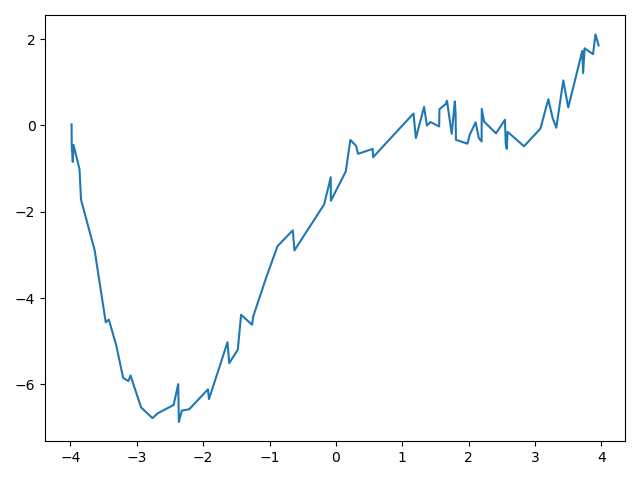
\includegraphics[width=12cm]{originalfunc1.png}
 \caption{Wykres aproksymowanej funkcji na podstawie plików treningowych 1}
 \vspace{-0.3cm}
 \label{originalfunc1}
\end{figure}

\begin{figure}[!htb]
 \centering
 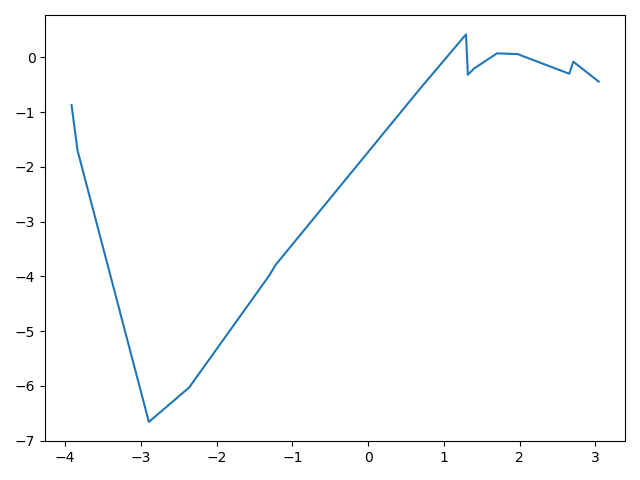
\includegraphics[width=12cm]{originalfunc2.png}
 \caption{Wykres aproksymowanej funkcji na podstawie plików treningowych 2}
 \vspace{-0.3cm}
 \label{originalfunc2}
\end{figure}

\begin{figure}[!htb]
 \centering
 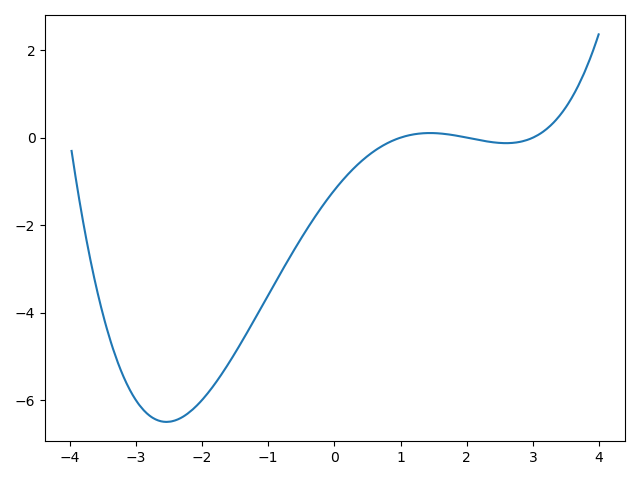
\includegraphics[width=12cm]{originalfunc3.png}
 \caption{Wykres aproksymowanej funkcji na podstawie plików testowych}
 \vspace{-0.3cm}
 \label{originalfunc3}
\end{figure}

\newpage
\section{Eksperymenty i wyniki} 

Wszystkie eksperymenty wykonujemy ustawiając numpy.random.seed() na wartość 0.

%%%%%%%%%%%%%%%%%%%%%%%%%%%%%%%%%%%%%%%%%%%%%%%%%%%%%%%%%%%%%%%%%%%%%%%%%%%%%%%%%%%%%%%%%%%%%%%%%%%%%%%%%%%%%%%%%
% PODROZDZIA� PT. EKSPERYMENT NR 1 
%%%%%%%%%%%%%%%%%%%%%%%%%%%%%%%%%%%%%%%%%%%%%%%%%%%%%%%%%%%%%%%%%%%%%%%%%%%%%%%%%%%%%%%%%%%%%%%%%%%%%%%%%%%%%%%%%

\subsection{Eksperyment nr 1}

W pierwszym eksperymencie postanowiliśmy przetestować możliwości\\ 
aproksymacji funkcji dla 1 neuronu w warstwie ukrytej.
\begin{figure}[!htb]
 \centering
 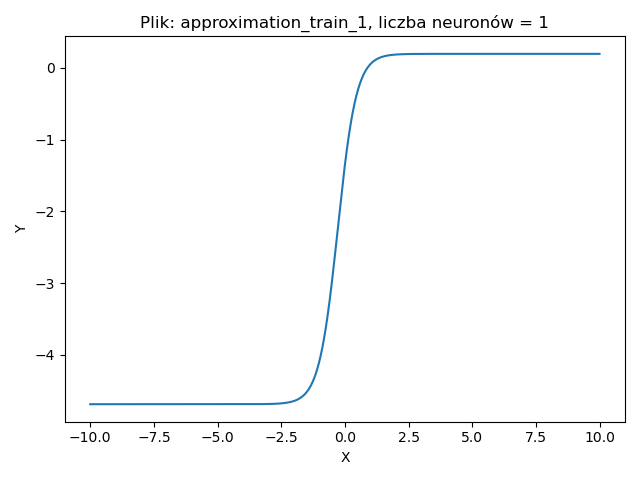
\includegraphics[width=12cm]{FunctionPlot1Neuron.png}
 \caption{Wykres apoksymowanej funkcji po 400 epokach}
 \vspace{-0.3cm}
 \label{WykresFun1}
\end{figure}



\begin{figure}[!htb]
 \centering
 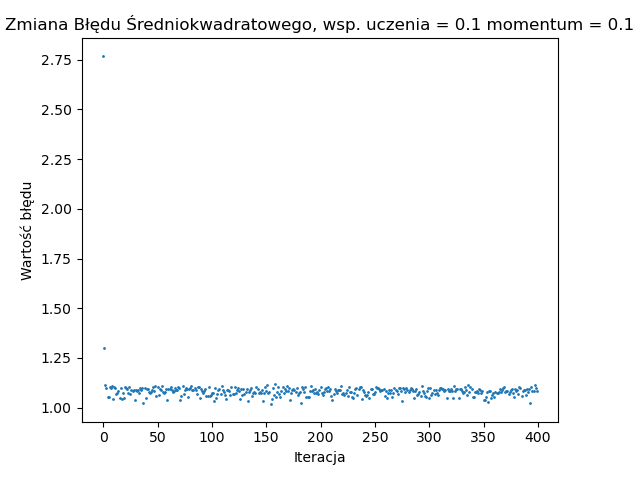
\includegraphics[width=12cm]{ZmianaBledu1Neuron.png}
 \vspace{-0.3cm}
 \caption{Wykres zmiany błędu dla 400 epok}
 \label{WykresBlad1}
\end{figure}

\newpage
Jak widać na rysunku Rys. \ref{WykresBlad1} błąd cały czas pozostawał taki sam.\\

Testując sieć na zbiorze testowym otrzymaliśmy błąd równy 0.536, który, chociaż duży okazuje się dwa razy mniejszy niż błędy uzyskiwane na zbiorze testowym.

Eksperyment ten powtórzylismy na drugim zbiorze treningowym. Wyniki okazały się bardzo zbliżone, błąd pozostawał taki sam podczas nauki a testując sieć na zbiorze testowym uzyskaliśmy duży błąd równy 0.840.  W próbie zachowania zwięzłości sprawozdania nie umieszczamy wyników.

\newpage

\subsection{Eksperyment nr 2}
W tym eksperymencie powtarzamy warunki z eksperymentu nr. 1, zwiększając jednak liczbę epok do tysiąca, tym razem dla 4 neuronów. 

Wyniki eksperymentów dla 2 i 3 neuronów byly badzo zbliżone do wyników poprzedniego eksperymentu, dlatego pomijamy je w sprawozdaniu.

\begin{figure}[!htb]
 \centering
 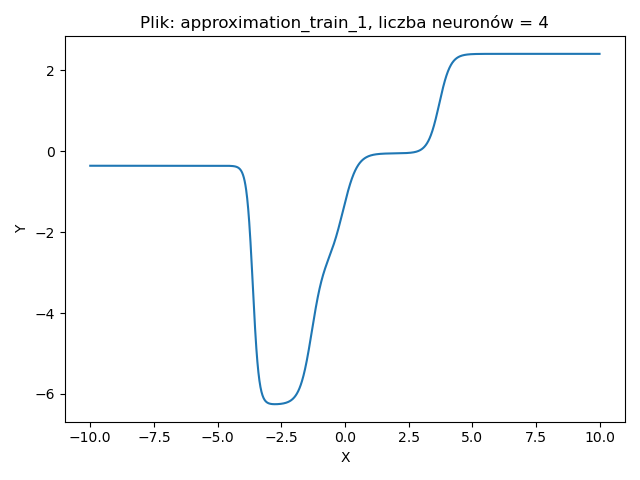
\includegraphics[width=12cm]{FunctionPlot4Neuron.png}
 \caption{Wykres apoksymowanej funkcji po 1000 epokach}
 \vspace{-0.3cm}
 \label{WykresFun2}
\end{figure}



\begin{figure}[!htb]
 \centering
 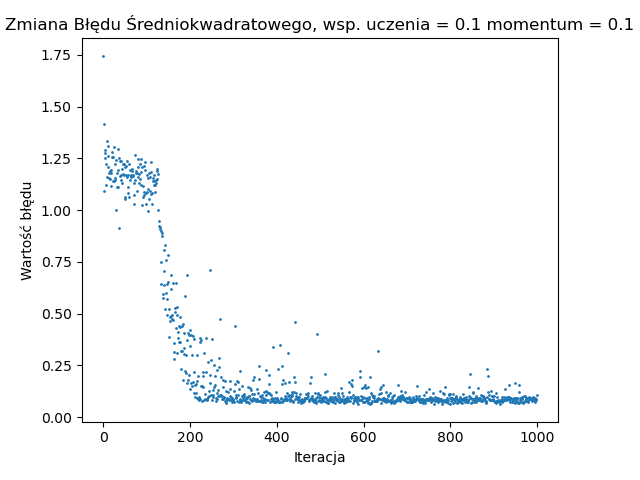
\includegraphics[width=12cm]{ZmianaBledu4Neuron.png}
 \vspace{-0.3cm}
 \caption{Wykres zmiany błędu dla 1000 epok}
 \label{WykresBlad2}
\end{figure}


\newpage
Jak widać na rysunku Rys. \ref{WykresBlad2} w tym eksperymencie nastąpiła 'nauka' sieci neuronowej.\\

Błąd na zbiorze testowym systematycznie malał aż do około 300 epoki, od którego momentu pozostawał w przybliżeniu nie zmieniony. Błąd ten był równy w przybliżeniu 0.13.

Testując sieć na zbiorze testowym otrzymaliśmy błąd równy 0.029, jest on dużo mniejszy niż ten otrzymywany dla ilości neuronów od 1 do 3. 

Analizując wykres aproksymowanej funkcji na rysunku Rys. \ref{WykresFun2} można zauważyć dużą różnicę względem poprzedniego eksperymentu.
\newpage
Eksperyment ten powtórzylismy na drugim zbiorze treningowym. 

\begin{figure}[!htb]
 \centering
 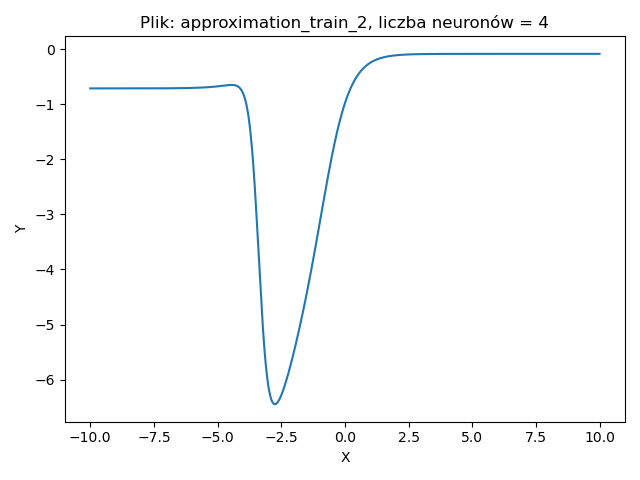
\includegraphics[width=12cm]{FunctionPlot4NeuronZbior2.png}
 \caption{Wykres apoksymowanej funkcji po 1000 epokach}
 \vspace{-0.3cm}
 \label{WykresFun3}
\end{figure}



\begin{figure}[!htb]
 \centering
 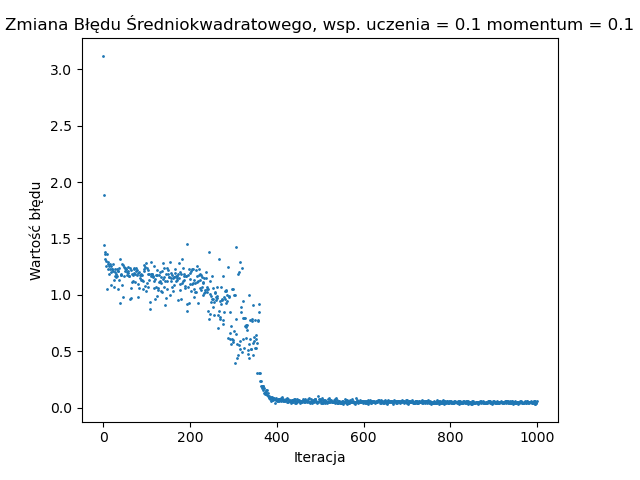
\includegraphics[width=12cm]{ZmianaBledu4NeuronZbior2.png}
 \vspace{-0.3cm}
 \caption{Wykres zmiany błędu dla 1000 epok}
 \label{WykresBlad3}
\end{figure}

\newpage
Widać zauważalną różnicę w nauce neuronu.

Otrzymany wykres funkcji na rysunku Rys. \ref{WykresFun3} jest zauważalnie mniej dokładny niż dla zbioru treningowego 1 na rysunku Rys. \ref{WykresFun2}.

Różnice widać też na wykresie zmian błędu średniokwadratowego. Dla drugiego zbioru testowego jak widać na rysunku Rys. \ref{WykresBlad3} zauważamy że po 'nauczeniu' się sieci około epoki 400 błąd pozostawał dużo bardziej stały niż dla pierwszego zbioru testowego, na rysunku Rys. \ref{WykresBlad2}.

Testując sieć na zbiorze testowym otrzymaliśmy błąd równy 0.150, a więc około 5 razy większy błąd niż dla zbioru treningowego 1. Możemy na podstawie tego przypuszczać że nauka sieci dla zbioru treningowego 1 postępuje lepiej.
\newpage

\subsection{Eksperyment nr 3}
W tym eksperymencie powtarzamy warunki z poprzedniego eksperymentu, z wykorzystaniem 6 neuronów w warstwie ukrytej.

\begin{figure}[!htb]
 \centering
 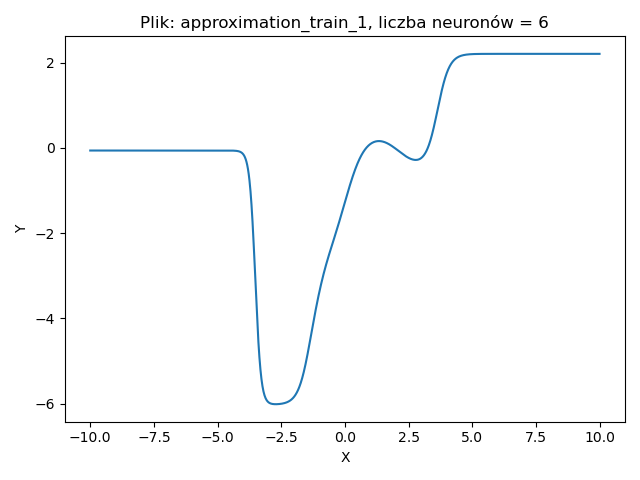
\includegraphics[width=12cm]{FunctionPlot6Neuron.png}
 \caption{Wykres apoksymowanej funkcji po 1000 epokach}
 \vspace{-0.3cm}
 \label{WykresFun4}
\end{figure}



\begin{figure}[!htb]
 \centering
 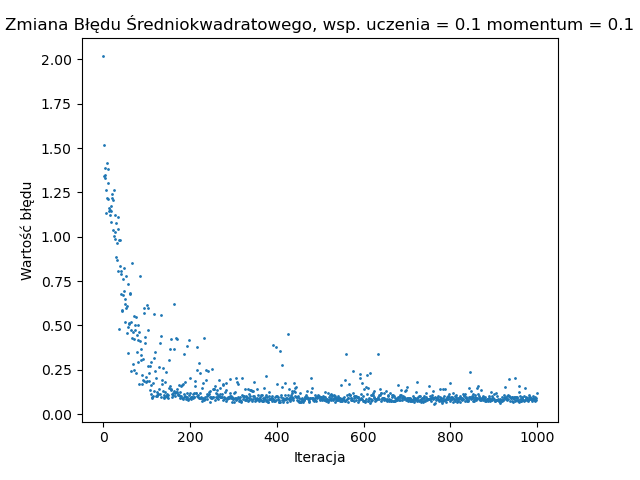
\includegraphics[width=12cm]{ZmianaBledu6Neuron.png}
 \vspace{-0.3cm}
 \caption{Wykres zmiany błędu dla 1000 epok}
 \label{WykresBlad4}
\end{figure}

\newpage
W tym eksperymencie jesteśmy w stanie zauważyć zmianę w szkicowanym wykresie funkcji w okolicach x = 2.5, jak widać na rysunku Rys. \ref{WykresFun4}.

Wykres zmiany błędu średniokwadratowego jest bardzo podobny do poprzedniego eksperymentu, dlatego jego komentarz pomijamy.

Mimo tego, że dokładność aproksymacji wydaje się być większa niż w poprzednik eksperymencie testując sieć na zbiorze testowym otrzymaliśmy błąd równy 0.072, więc zauważalnie większy, bo ponad trzy krotnie, niż w eksperymencie dla 4 neuronów. 

Analizując wykres aproksymowanej funkcji na rysunku Rys. \ref{WykresFun2} można zauważyć dużą różnicę względem poprzedniego eksperymentu.
\newpage
Eksperyment ten powtórzylismy na drugim zbiorze treningowym. 

\begin{figure}[!htb]
 \centering
 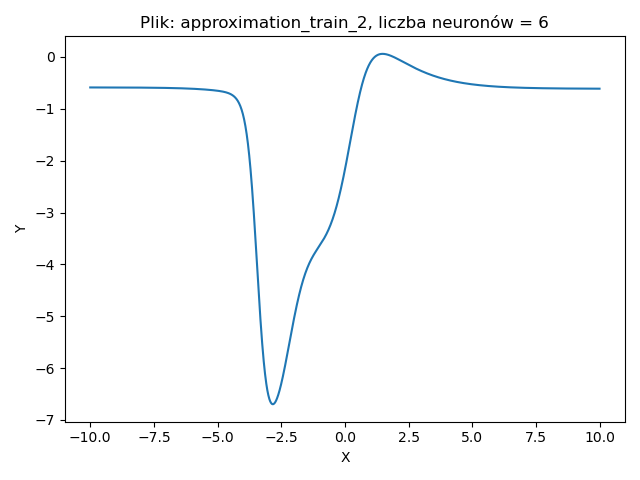
\includegraphics[width=12cm]{FunctionPlot6NeuronZbior2.png}
 \caption{Wykres apoksymowanej funkcji po 1000 epokach}
 \vspace{-0.3cm}
 \label{WykresFun5}
\end{figure}



\begin{figure}[!htb]
 \centering
 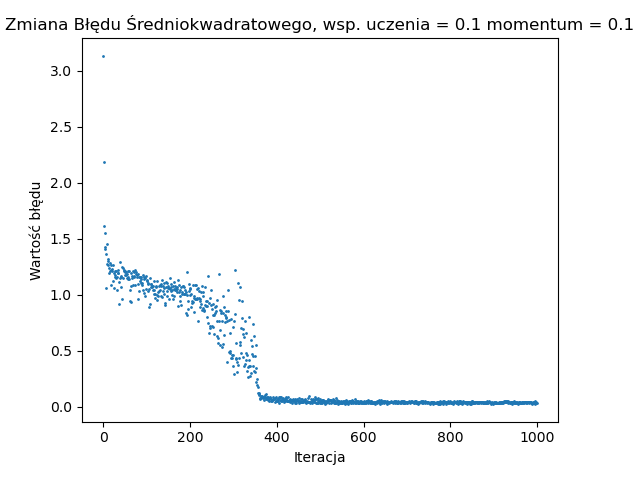
\includegraphics[width=12cm]{ZmianaBledu6NeuronZbior2.png}
 \vspace{-0.3cm}
 \caption{Wykres zmiany błędu dla 1000 epok}
 \label{WykresBlad5}
\end{figure}

\newpage
Wykres zmiany błędu średniokwadratowego jest bardzo podobny do poprzedniego eksperymentu, dlatego jego komentarz pomijamy.

Ponownie, otrzymany wykres funkcji na rysunku Rys. \ref{WykresFun5} jest zauważalnie mniej dokładny niż dla zbioru treningowego 1 na rysunku Rys. \ref{WykresFun4}.

Testując sieć na zbiorze testowym otrzymaliśmy błąd równy 0.228, a więc podobnie jak dla zbioru treningowego 1 wraz z wzrostem ilości neuronów wzrósł błąd.
\newpage

\subsection{Eksperyment nr 4}
Ponawiamy poprzednią konfigurację dla 7 neuronów.

\begin{figure}[!htb]
 \centering
 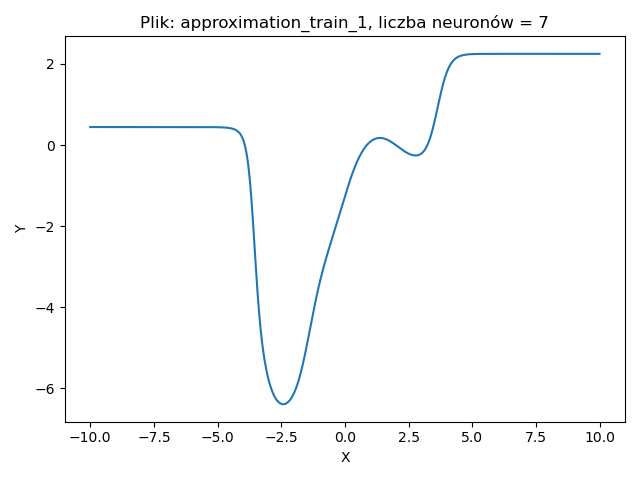
\includegraphics[width=12cm]{FunctionPlot7Neuron.png}
 \caption{Wykres apoksymowanej funkcji po 1000 epokach}
 \vspace{-0.3cm}
 \label{WykresFun6}
\end{figure}



\begin{figure}[!htb]
 \centering
 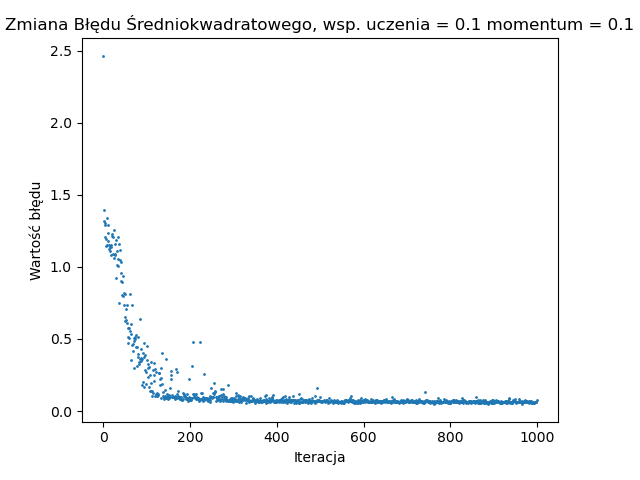
\includegraphics[width=12cm]{ZmianaBledu7Neuron.png}
 \vspace{-0.3cm}
 \caption{Wykres zmiany błędu dla 1000 epok}
 \label{WykresBlad6}
\end{figure}

\newpage

Zauważamy dużą zmianę w wykresie błędu średniokwadratowego, jak widać na rysunku Rys. \ref{WykresBlad6} dla 7 neuronów po osiągnięciu momentu kiedy błąd średniokwadratowy dla kolejnych epok się ustabilizował, w odróżnieniu od poprzedniej próby, rysunek Rys. \ref{WykresBlad4}, nie pojawiają się żadne epoki dla których zauważylibyśmy duże zmiany błędu średniokwadratowego. Sam błąd również ustabilizował się na bardzo niskich wartościach, bo bliskich 0.07. 

W wykresie funkcji brak zauważalnych zmian względem poprzedniego eksperymentu.

Testując sieć na zbiorze testowym otrzymaliśmy błąd równy 0.075, a więc podobnie jak w poprzednim eksperymencie.

Dla drugiego zbioru testowego nie zaobserwowaliśmy zauważalnych różnic względem poprzedniego eksperymentu.

\newpage

\subsection{Eksperyment nr 5}
Znowu powtarzamy te same warunki jak w poprzednim eksperymencie.
Eksperyment wykonujemy dla 20 neuronów, nie zauważyliśmy widocznych zmian dla mniejszych ilości neronów, więc tamte eksperymenty pomijamy.


\begin{figure}[!htb]
 \centering
 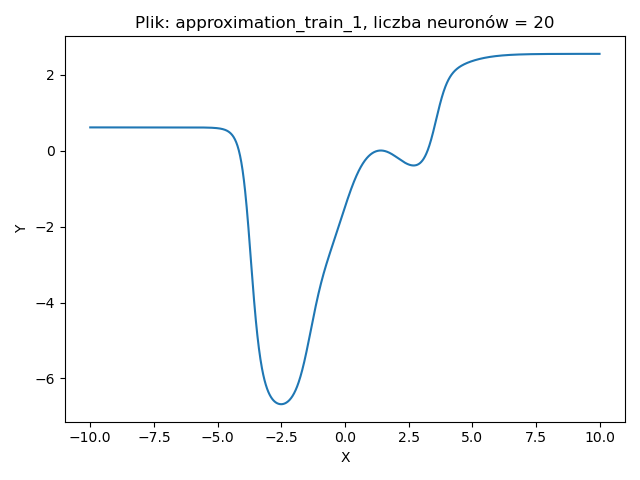
\includegraphics[width=12cm]{FunctionPlot20Neuron.png}
 \caption{Wykres apoksymowanej funkcji po 1000 epokach}
 \vspace{-0.3cm}
 \label{WykresFun7}
\end{figure}



\begin{figure}[!htb]
 \centering
 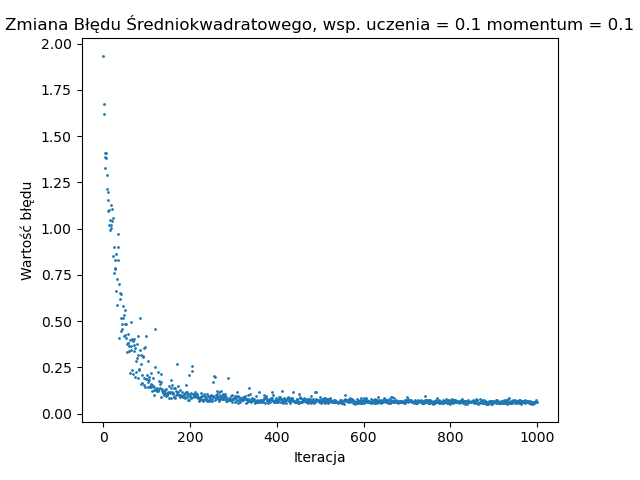
\includegraphics[width=12cm]{ZmianaBledu20Neuron.png}
 \vspace{-0.3cm}
 \caption{Wykres zmiany błędu dla 1000 epok}
 \label{WykresBlad7}
\end{figure}


\newpage
Wyniki są bardzo zbliożone do poprzednich eksperymentów, z wyjątkiem błędu otrzymanego testując aproksymację na zbiorze testowym. Błąd ten okazał się być równy zaledwie 0.033, a więc był on najmniejszy poza błędem otrzymanym dla 4 neuronów. Błąd ten malał powoli dla każdego dodanego neuronu, jednak była to jedyna zauważalna różnica pomiędzy kolejnymi dodanymi neuronami więc te eksperymenty pomijamy.

Otrzymane rezultaty zachęciły nas do sprawdzenia eksperymentu dla 4 neuronów przy innym 'seedzie' losowego generatora. Przy seedzie = 1 otrzymaliśmy błąd około 0.1 na zbiorze testowym, więc według nas to, że błąd dla 4 neuronów okazał się tak mały było przypadkiem, a sam błąd maleje, choć powoli, dla coraz większych ilości neuronów. Dla porównania błąd dla seedu = 1 dla 20 neuronów okazał się równy 0.017.

Dla pliku treningowego nr 2 nie zauważylismy dużych różnic względem poprzedniego eksperymentu więc te wyniki pomijamy.
\newpage

\subsection{Eksperyment nr 6}
W tym eksperymencie analizujemy wpływ współczynniku uczenia i momentum na wyniki.

Ostatnią zauważalną zmianę w przebiegu nauki zaobserwowaliśmy dla 7 neuronów, więc dla takiej ilości przeprowadzamy te eksperymenty.

\begin{figure}[!htb]
 \centering
 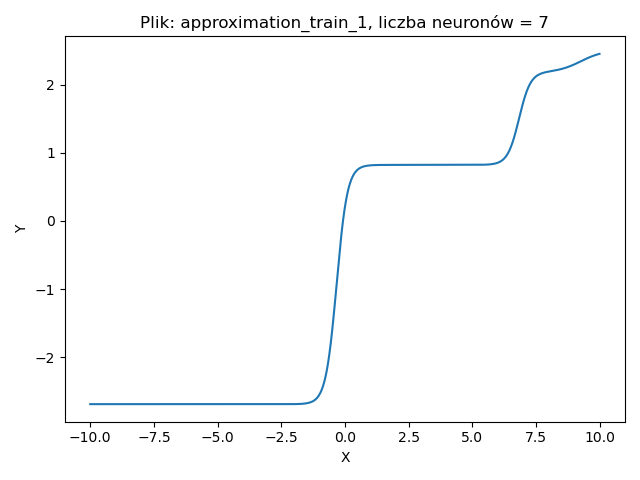
\includegraphics[width=12cm]{FunctionPlot7Neuronmomentum08.png}
 \caption{Wykres apoksymowanej funkcji po 1000 epokach}
 \vspace{-0.3cm}
 \label{WykresFun8}
\end{figure}



\begin{figure}[!htb]
 \centering
 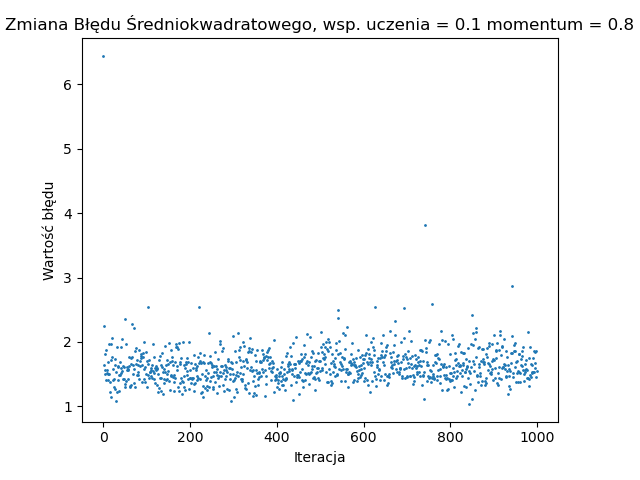
\includegraphics[width=12cm]{ZmianaBledu7Neuronmomentum08.png}
 \vspace{-0.3cm}
 \caption{Wykres zmiany błędu dla 1000 epok}
 \label{WykresBlad8}
\end{figure}
\newpage
Jak widać na rysunku Rys. \ref{WykresBlad8} dla momentum = 0.8 proces nauki sieci nie udał się. Otrzymany błąd dla zbioru testowego jest równy 1.6.

\begin{figure}[!htb]
 \centering
 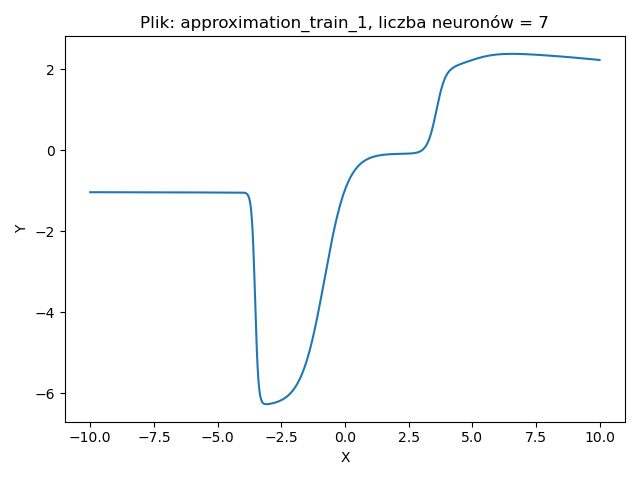
\includegraphics[width=12cm]{FunctionPlot7Neuronmomentum05.png}
 \caption{Wykres apoksymowanej funkcji po 1000 epokach}
 \vspace{-0.3cm}
 \label{WykresFun9}
\end{figure}

\begin{figure}[!htb]
 \centering
 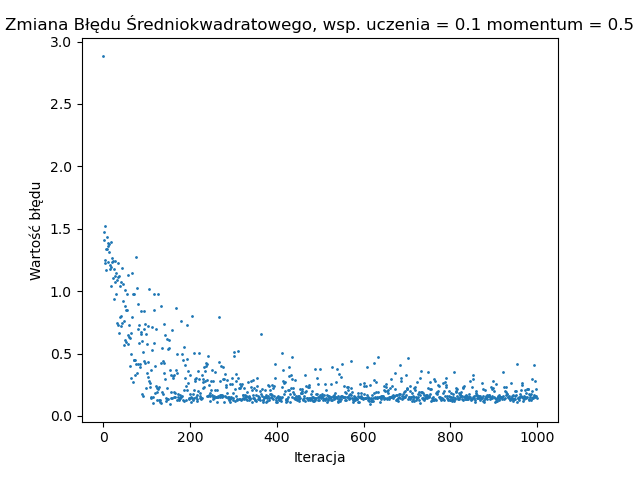
\includegraphics[width=12cm]{ZmianaBledu7Neuronmomentum05.png}
 \vspace{-0.3cm}
 \caption{Wykres zmiany błędu dla 1000 epok}
 \label{WykresBlad9}
\end{figure}


\newpage
Możemy zauważyć na rysunku Rys. \ref{WykresBlad9}, że dla momentum = 0.5 nauka już przebiega, chociaż zauważalnie gorzej niż przy momentum = 0.1.
Mimo tego, że błąd poczas nauki okazywał się ' skoczny', to błąd na zbiorze testowym = 0.06. Sprawdzenie dla seedu = 1 pokazało, że był to przypadek, tam błąd = 0.123
\newpage


\begin{figure}[!htb]
 \centering
 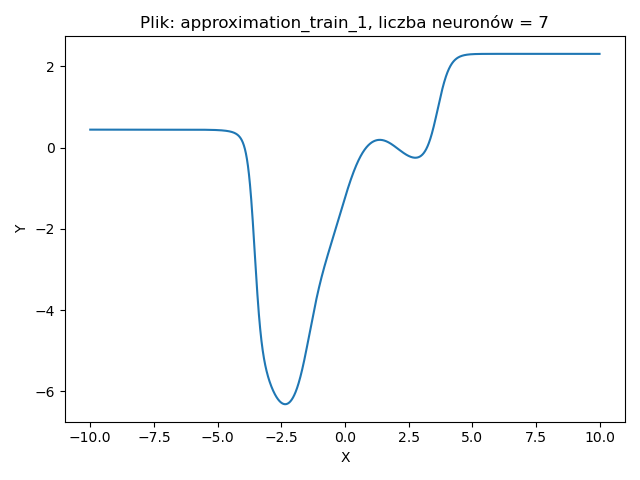
\includegraphics[width=12cm]{FunctionPlot7Neuronmomentum00.png}
 \caption{Wykres apoksymowanej funkcji po 1000 epokach}
 \vspace{-0.3cm}
 \label{WykresFun10}
\end{figure}

\begin{figure}[!htb]
 \centering
 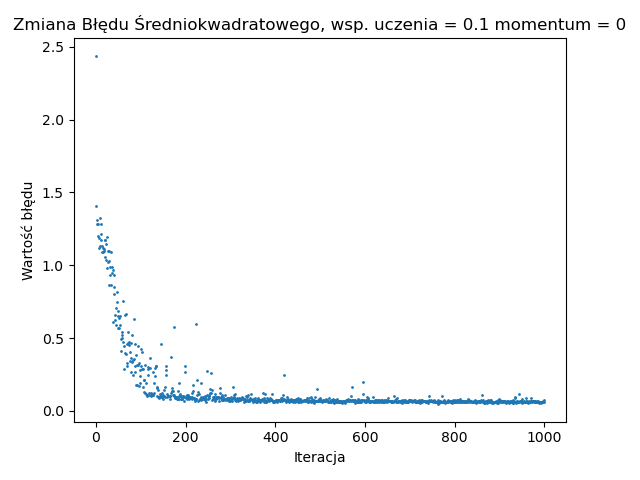
\includegraphics[width=12cm]{ZmianaBledu7Neuronmomentum00.png}
 \vspace{-0.3cm}
 \caption{Wykres zmiany błędu dla 1000 epok}
 \label{WykresBlad10}
\end{figure}


\newpage
Wyeliminowanie momentum wydaje się dawać najlepsze rezultaty. Błąd na zbiorze testowym = 0.076, a wykres błędu na zbiorze treningowym wygląda 'dobrze'.



\begin{figure}[!htb]
 \centering
 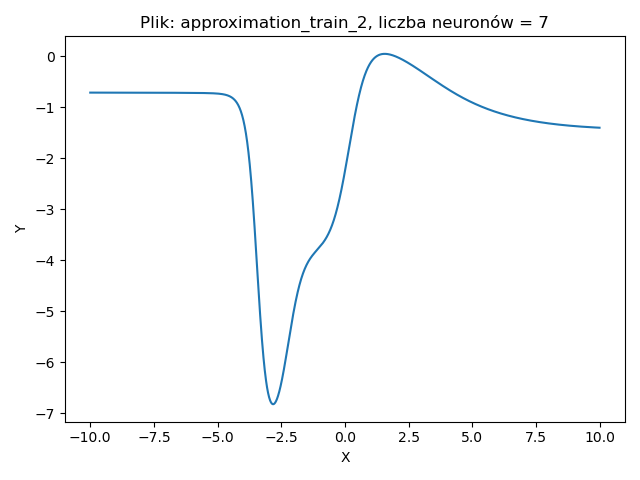
\includegraphics[width=12cm]{FunctionPlot7Neuronmomentum05DWA.png}
 \caption{Wykres apoksymowanej funkcji po 1000 epokach}
 \vspace{-0.3cm}
 \label{WykresFun11}
\end{figure}

\begin{figure}[!htb]
 \centering
 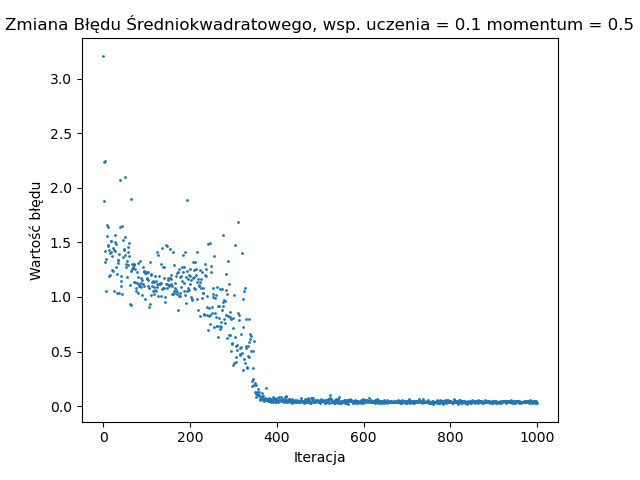
\includegraphics[width=12cm]{ZmianaBledu7Neuronmomentum05DWA.png}
 \vspace{-0.3cm}
 \caption{Wykres zmiany błędu dla 1000 epok}
 \label{WykresBlad11}
\end{figure}

\newpage

Inaczej sytacja wygląda dla drugiego zbioru treningowego. Tutaj, jak widać na Rysunku Rys. \ref{WykresBlad11} wykres zmiany błędu dla drugiego zestawu treningowego wygląda ' dobrze ', również wykres funkcji zgadza się z oczekiwanym a błaD na zbiorze testowym, równy 0.27 jest zbliżony do tego otrzmanego dla momentum = 0.1.



\begin{figure}[!htb]
 \centering
 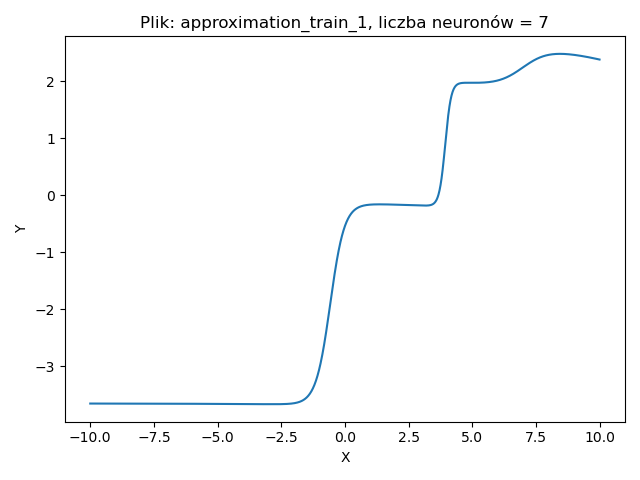
\includegraphics[width=12cm]{FunctionPlot7Neuronucz05.png}
 \caption{Wykres apoksymowanej funkcji po 1000 epokach}
 \vspace{-0.3cm}
 \label{WykresFun12}
\end{figure}

\begin{figure}[!htb]
 \centering
 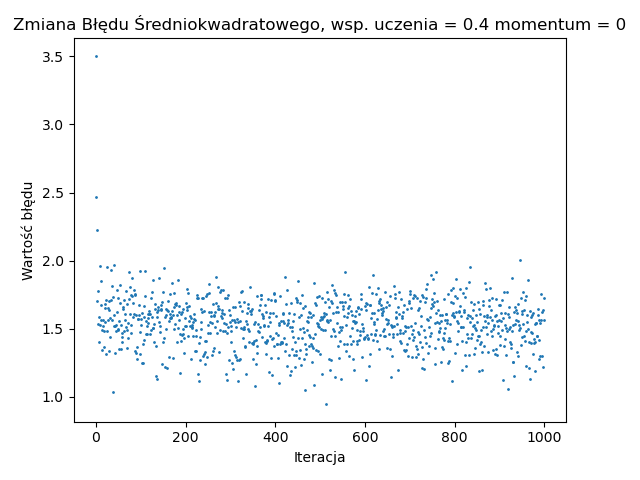
\includegraphics[width=12cm]{ZmianaBledu7Neuronucz05.png}
 \vspace{-0.3cm}
 \caption{Wykres zmiany błędu dla 1000 epok}
 \label{WykresBlad12}
\end{figure}
\newpage
Zawuważalnie, wykres na rysunku Rys. \ref{WykresFun12} wygląda 'źle', po wykresie zmiany błędu widzimy, że nauka nie nastapiła.
Błąd na zbiorze testowym = 0.81.
\newpage
\section{Wnioski}

Zauważamy, że przeprowadzona przez nas aproksymacja wykorzystująca sieć neuronową jest poprawna. W najlepszych przypadkach otrzymujemy przybliżenia wartości funkcji dla testowanego zbioru o średnim błędzie bliskim 0.02. \\ Zauważamy również, że niskie wartości momentum i współczynniku uczenia oraz duża liczba neuronów daje nam najlepsze rezultaty.\\ Zauważamy, że do odpowiedniego odwzorowania tej funkcji potrzebujemy przynajmniej 7 neuronów, a nauka na większym, pierwszym, zbiorze pozwala lepiej przybliżyć wartości punktów nie należąchych do tego zbioru.


%%%%%%%%%%%%%%%%%%%%%%%%%%%%%%%%%%%%%%%%%%%%%%%%%%%%%%%%%%%%%%%%%%%%%%%%%%%%%%%%%%%%%%%%%%%%%%%%%%%%%%%%%%%%%%%%%
% PODROZDZIA� PT. ZALACZNIKI
%%%%%%%%%%%%%%%%%%%%%%%%%%%%%%%%%%%%%%%%%%%%%%%%%%%%%%%%%%%%%%%%%%%%%%%%%%%%%%%%%%%%%%%%%%%%%%%%%%%%%%%%%%%%%%%%%



%%%%%%%%%%%%%%%%%%%%%%%%%%%%%%%%%%%%%%%%%%%%%%%%%%%%%%%%%%%%%%%%%%%%%%%%%%%%%%%%%%%%%%%%%%%%%%%%%%%%%%%%%%%%%%%%%
% BIBLIOGRAFIA
%%%%%%%%%%%%%%%%%%%%%%%%%%%%%%%%%%%%%%%%%%%%%%%%%%%%%%%%%%%%%%%%%%%%%%%%%%%%%%%%%%%%%%%%%%%%%%%%%%%%%%%%%%%%%%%%%

\renewcommand\refname{Bibliografia}
\bibliographystyle{plain}
\bibliography{bibliografia_wzor}

\end{document}
